
\appendix

\chapter{Adversarial ensemble evaluation} \label{appendix:adversarial-ensemble-plots}

This appendix is an extension of the out-of-distribution evaluation experiment of section \ref{experiment:OOD-evaluation}. The evaluation of adversarial ensembles trained on white noise attack is shared in figure \ref{fig:adversarial-evaluation-training-ensemble-noise}. Figure \ref{fig:adversarial-evaluation-training-ensemble-udp} contains the equivalent results for the UDP attack. As stated in section \ref{experiment:OOD-evaluation}, robustness is assessed via ensemble attacks aggregated using the $mean$, $random$ and $max$ functions.

\begin{figure}[htbp]
    \begin{subfigure}{\textwidth}
      \centering
      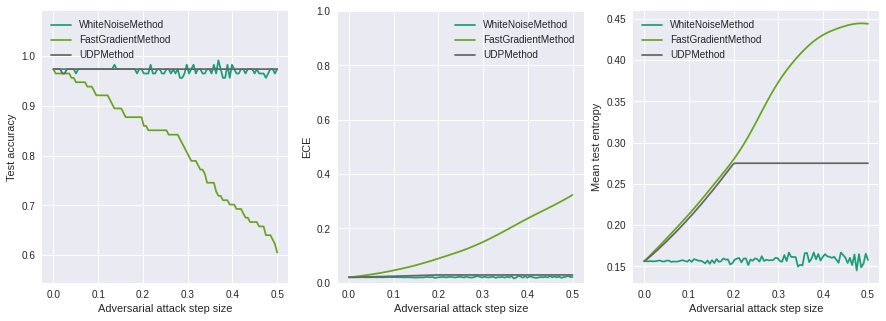
\includegraphics[width=\linewidth]{figures/eval/eval_adv_uq_train_ensemble_noise_mean.png}
      \caption{Evaluation on ensemble $mean$ attacks.}
    \end{subfigure}
    % \begin{subfigure}{\textwidth}
    %  \centering
    %  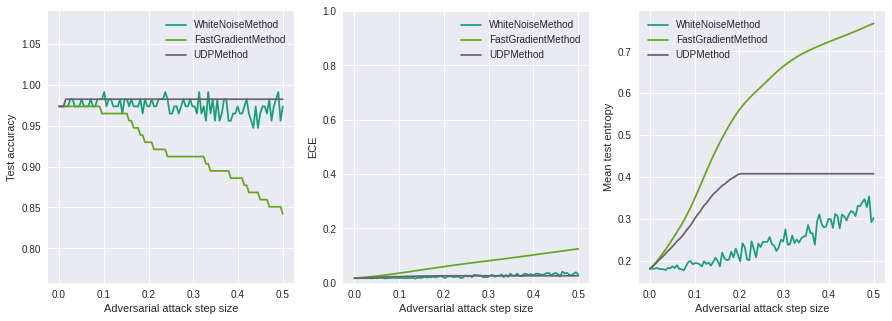
\includegraphics[width=\linewidth]{figures/eval/eval_adv_uq_train_ensemble_fgsm_first.png}
    %  \caption{Adversarial training on the ensemble first FGSM attack}
    %\end{subfigure}
     \begin{subfigure}{\textwidth}
      \centering
      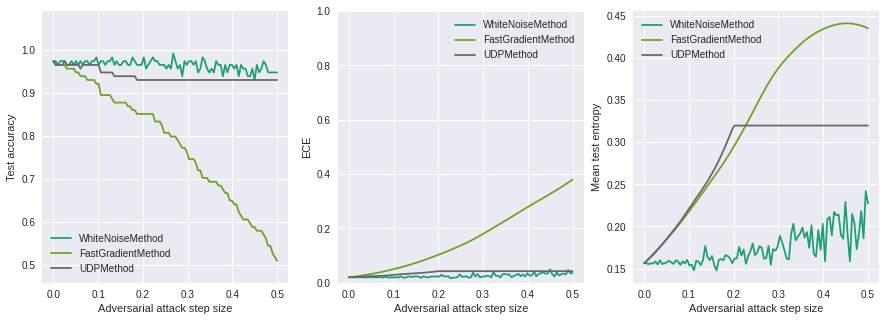
\includegraphics[width=\linewidth]{figures/eval/eval_adv_uq_train_ensemble_noise_random.png}
      \caption{Evaluation on ensemble $random$ attacks.}
    \end{subfigure}
    \begin{subfigure}{\textwidth}
      \centering
      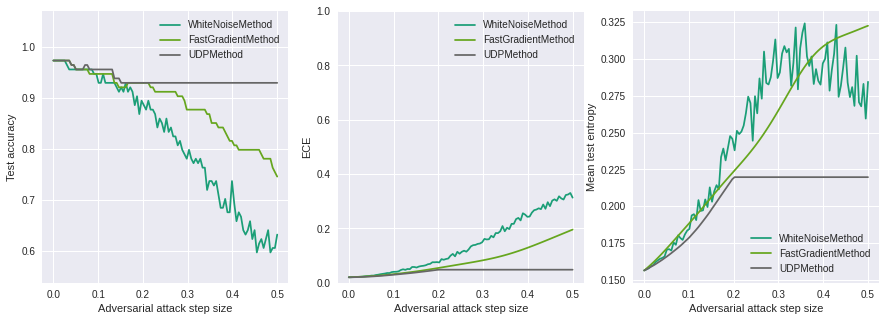
\includegraphics[width=\linewidth]{figures/eval/eval_adv_uq_train_ensemble_noise_max.png}
      \caption{Evaluation on ensemble $max$ attacks.}
    \end{subfigure}
    \caption{Evaluation of an Adversarial ensemble composed of 10 Logistic Regression models (breast cancer dataset). It is trained only on the white noise attack.}
    \label{fig:adversarial-evaluation-training-ensemble-noise}
\end{figure}

\begin{figure}[htbp]
    \begin{subfigure}{\textwidth}
      \centering
      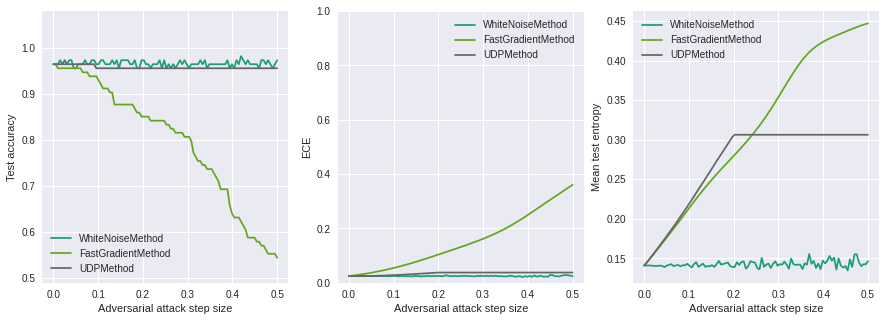
\includegraphics[width=\linewidth]{figures/eval/eval_adv_uq_train_ensemble_udp_mean.png}
       \caption{Evaluation on ensemble $mean$ attacks.}
    \end{subfigure}
    % \begin{subfigure}{\textwidth}
    %  \centering
    %  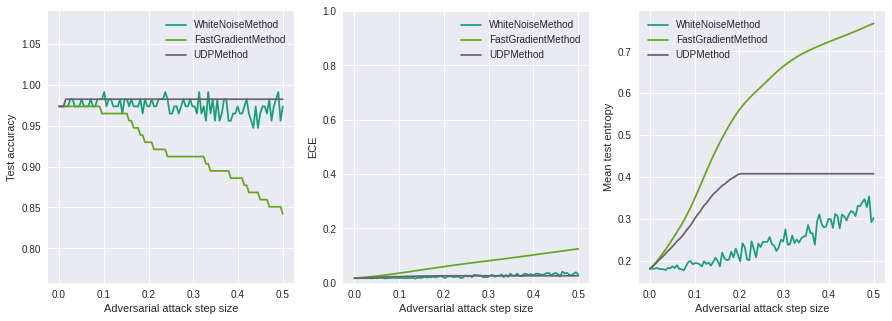
\includegraphics[width=\linewidth]{figures/eval/eval_adv_uq_train_ensemble_fgsm_first.png}
    %  \caption{Adversarial training on the ensemble first FGSM attack}
    %\end{subfigure}
     \begin{subfigure}{\textwidth}
      \centering
      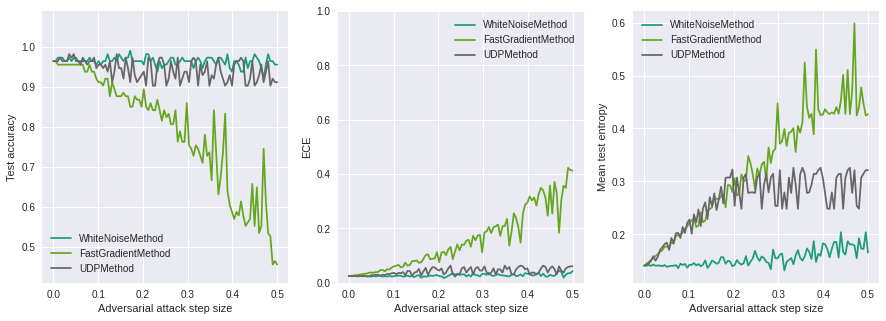
\includegraphics[width=\linewidth]{figures/eval/eval_adv_uq_train_ensemble_udp_random.png}
       \caption{Evaluation on ensemble $random$ attacks.}
    \end{subfigure}
    \begin{subfigure}{\textwidth}
      \centering
      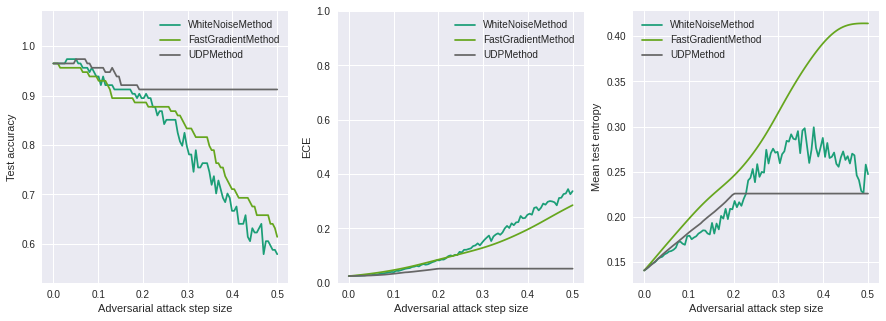
\includegraphics[width=\linewidth]{figures/eval/eval_adv_uq_train_ensemble_udp_max.png}
      \caption{Evaluation on ensemble $max$ attacks.}
    \end{subfigure}
    \caption{Evaluation of an Adversarial ensemble composed of 10 Logistic Regression models (breast cancer dataset). It is trained only on the UDP attack.}
    \label{fig:adversarial-evaluation-training-ensemble-udp}
\end{figure}


\chapter{Named Entity Recognition fine-tuned on the SAR dataset} \label{appendix:custom-ner-sar}

In section \ref{experiment:G2T-raw-performance}, the performance and faithfulness of the graph-to-text models are evaluated. For the SAR dataset, a custom, fined-tuned NER model is mentioned. This section provides some information about the latter. 


The model is based on the RoBERTa transformer architecture and fine-tuned using the spaCy library. It was introduced in 2022 by D. Tekin, a colleague at Oracle, for his work on 
Knowledge Graph Construction from Unstructured Text using Named Entity Recognition, Relation Extraction, and Coreference Resolution. The performance of his approach is reported in table \ref{tab:NER-doga-performance} for the CoNLL-2004\cite{CoNLL4},  SciERC\cite{SciERC} and SAR datasets for comparison purposes.


\begin{table}[!ht]
    \centering
    \begin{tabular}{llcc}
    \toprule
        Dataset        & Model      & Micro-F1 & Macro-F1  \\
    \midrule
        CoNLL-2004     & Wang and Lu.,2020\cite{Lu2020} & 90.10 & 86.90 \\
        CoNLL-2004     & Tekin, 2022 & 90.34 & 87.19 \\
        SciERC         &  Luan et al.\cite{SciERC}, 2018 & 64.20 & --- \\
        SciERC         & Tekin, 2022 & 66.80 & --- \\
        SAR            & Tekin, 2022 & 88.82 & --- \\             
         \bottomrule
    \end{tabular}
    \caption{Performance of various NER models.}
    \label{tab:NER-doga-performance}
\end{table}

